% !TeX encoding = utf8
\documentclass[german,aspectratio=169]{beamer}

\usepackage{beamerthemeHM-blue} 
\input{./../../includes/ColorDefinitions}
\input{./../../includes/packages}
\input{./../../includes/meta}
\input{./../../includes/commands}
\input{./../../includes/listing-style}
\lstset{style=ipython}

\graphicspath{{./figs/}}
\setbeamercolor{alerted text}{fg=red}
\title{Feedward Neural Networks}
\subtitle{}
\author{\href{mailto:zoennchen.benedikt@hm.edu}{\textbf{Benedikt Z\"onnchen}}} 
\date{\today}
%\setdefaultlanguage[spelling=new]{german}

\begin{document}
	
\begin{frame}
	\titlepage
\end{frame}

\section{Motivation}
\begin{frame}
	\frametitle{Motivation}
	\begin{Beispiel}[Problem]
		Wir wollen die Art eines Kleidungsstücks auf einem Bild erkennen. Wie lösen wir diese Aufgabe?
	\end{Beispiel}
\end{frame}

\begin{frame}
	\frametitle{Motivation}
	Wir wollen eine Funktion $h$, die uns für eine Eingabe $\xx$ (ein $m \times n$-Pixelbild) ausgibt, welches Kleidungsstück $\xx$ ist.
	\begin{center}
		$h(\xx) = \text{'T-Shirt'}$
	\end{center}
	$h : [0;1]^{m \times n} \rightarrow \{\text{'T-Shirt'}, \text{'Pullover'}, \ldots, \text{'Sneaker'} \}$.
\end{frame}


\begin{frame}
	\frametitle{Motivation}
	\begin{enumerate}[label=(\arabic*)]
		\item Klassisch: Konstruiere Algorithmus $h$ der die Antwort berechnet
		\item \hl{Überwachtes Maschinelles Lernen}: Konstruiere eine \term{parametrisierbaren} Algorithmus $h_\theta$, dessen \term{Parameter} $\theta$ durch Antworten kalibriert werden 	
	\end{enumerate}
	\begin{figure}
		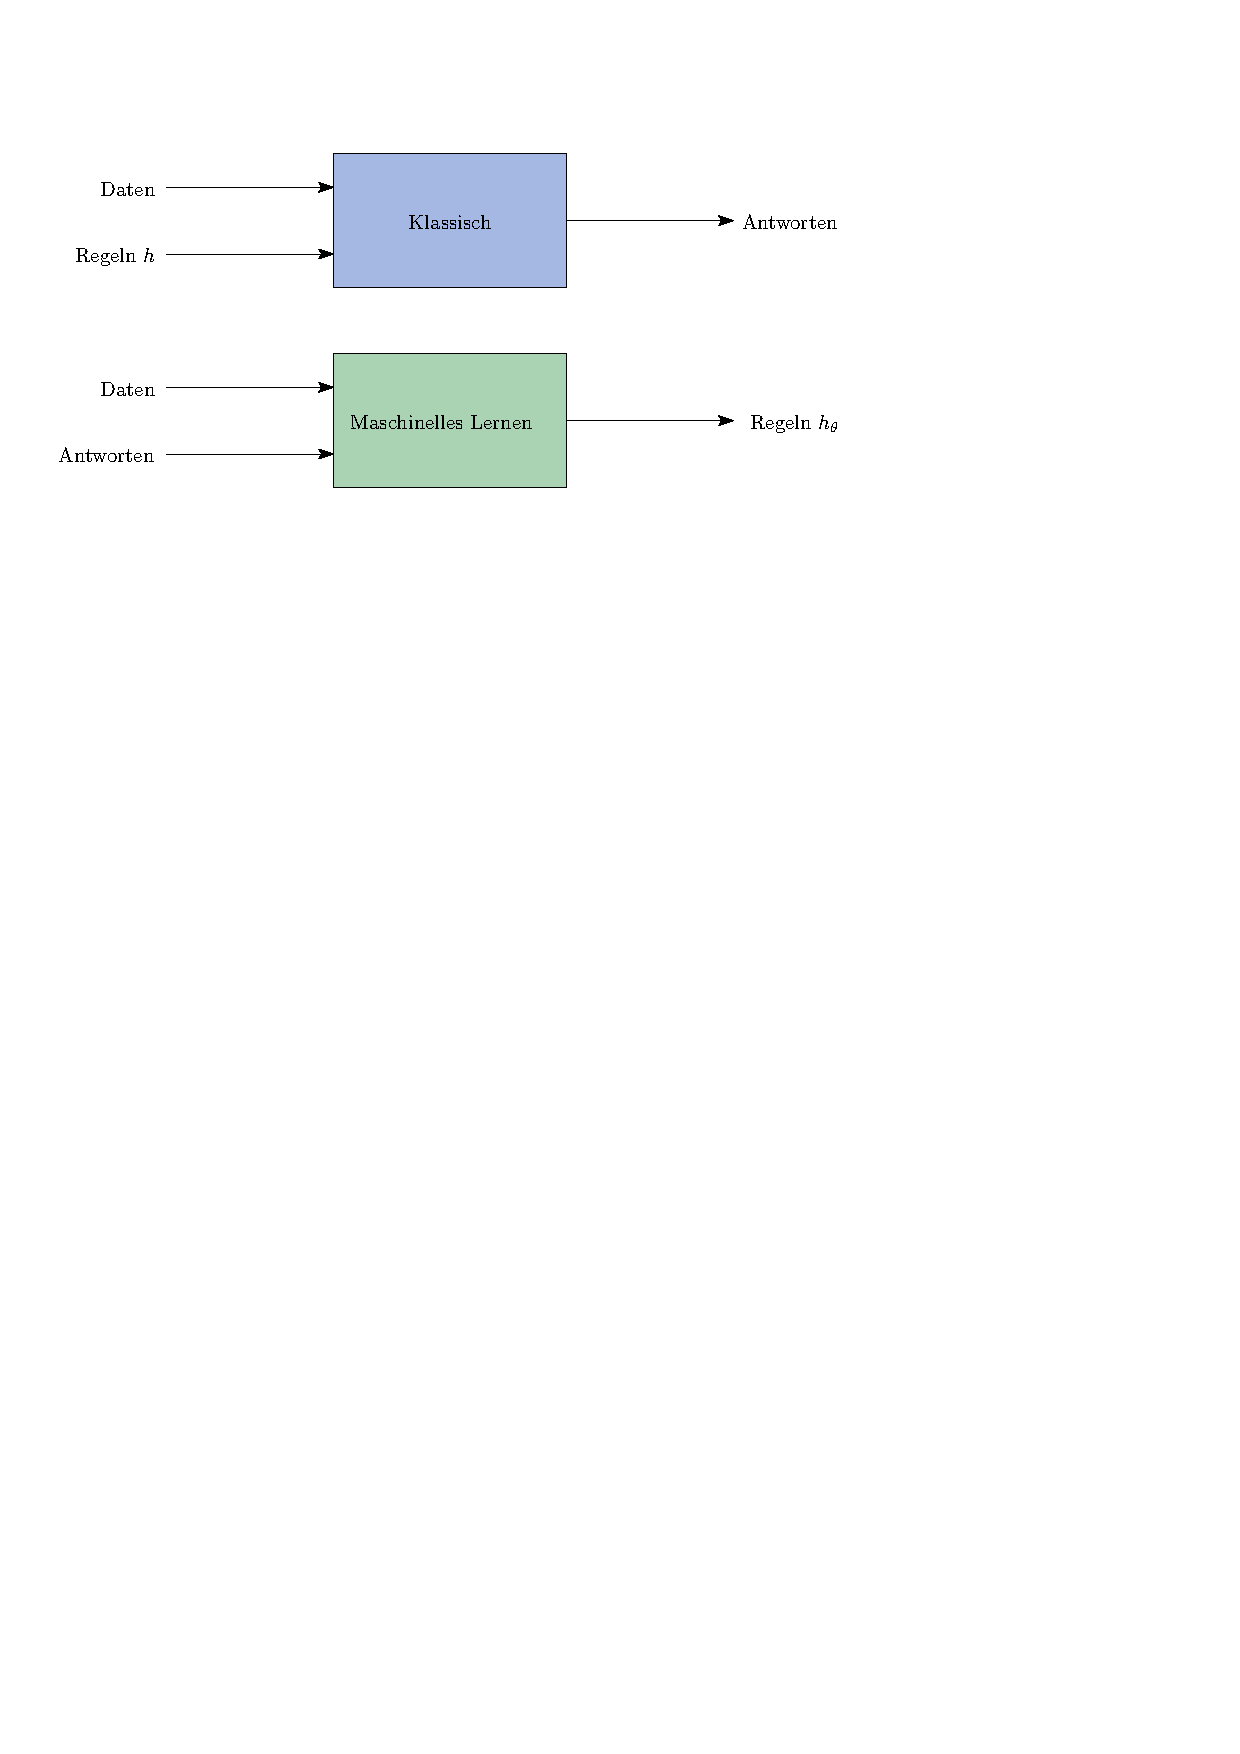
\includegraphics[width=0.65\textwidth]{classic-vs-ml}
	\end{figure}
	Diese Kalibrierung nennen wir auch \term{Lernen}.
\end{frame}

\begin{frame}
	\frametitle{Motivation}
	\begin{definition}[Maschinelles Lernen]
		Ein Computerprogramm lernt von der Erfahrung $\experience$ hinsichtlich einer Aufgabe $\task$ und einem Leistungskriterium $\criteria$, 
		wenn sich seine Leistung bei der Durchführung von $\task$, wie sie von $\criteria$ gemessen wurde, mit der Erfahrung $\experience$ verbessert \cite{Mitchell1997}.   
	\end{definition}
	%	\begin{block}{Problem}
		%		Given 8 attributes (longitude, latitude, house age, rooms, bedrooms, population, households, income), we want to predict the (mean) \textit{house value}.
		%	\end{block}
\end{frame}

\section{Computationalism}
\begin{frame}
	\frametitle{Computationalism}
	\begin{quoting}
		``Brains have the same computational capacity as Turing machines.''\\ -- Hilary Putnam (1975)
	\end{quoting}
\end{frame}

\begin{frame}
	\frametitle{Computationalism}
Falls dies zutrifft ist es zumindest theoretisch möglich ein funktionierendes Gehirn wie das unsere aus einem ganz anderen Material zu bauen.\\
\vspace{0.5cm}
$\Rightarrow$ Es kommt rein auf die 'Software' an, welche die (mentalen) Zustände berechnet.\\
\vspace{0.5cm}
Wichtiges Gedankenexperiment: \hll{Das chinesische Zimmer}.
\end{frame}


\begin{frame}
	\frametitle{Computationalism}
	\framesubtitle{The Symbol-system Paradigm}
	\hl{Das Gehirn als automatisches formales System} (Hypothese) \cite{McLaughlin2008}:
	\begin{enumerate}[label=$\bullet$]
		\item Unsere mentale Fähigkeiten lassen sich zumindest teilweise auf automatische formale Systeme zurückführen.
		\item Mentale Zustände sind Repräsentationen
		\item Es gibt eine Art \term{Sprache des Denkens}
	\end{enumerate}
	\vspace{1cm}
	Schach ist beispielsweise ein formales System.
	\begin{tikzpicture}[remember picture,overlay]
		\node[xshift=-5cm,yshift=-5.5cm] at (current page.north east){%
			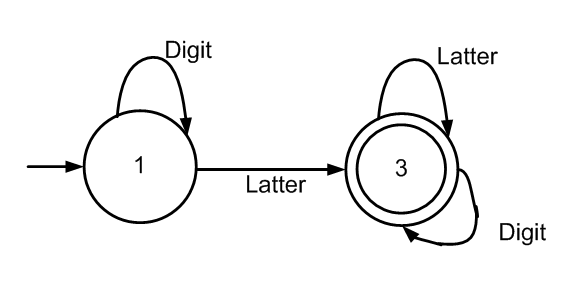
\includegraphics[width=0.35\textwidth]{automata}};
	\end{tikzpicture}
\end{frame}

\begin{frame}
	\frametitle{Computationalism}
	\framesubtitle{The Connectionist Computational Paradigm}
	\hl{Das Gehirn als vernetztes Netzwerk} (Hypothese) \cite{McLaughlin2008}:
	\begin{enumerate}[label=$\bullet$]
		\item Untersuchung von funktionalen Architekturen die durch neuronale Netze inspiriert sind
		\item Anstatt einer zentralen Recheneinheit gibt es ein Netzwerk aus Knoten
		\item Jeder Knoten nimmt an der Informationsverarbeitung teil (verteilt und parallel) 
	\end{enumerate}
	
	\begin{tikzpicture}[remember picture,overlay]
		\node[xshift=-5cm,yshift=-7.5cm] at (current page.north east){%
			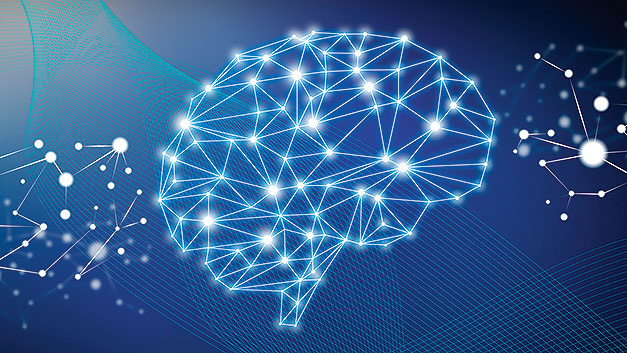
\includegraphics[width=0.3\textwidth]{neurons}};
	\end{tikzpicture}

	\begin{tikzpicture}[remember picture,overlay]
		\node[xshift=-10cm,yshift=-7.5cm] at (current page.north east){%
			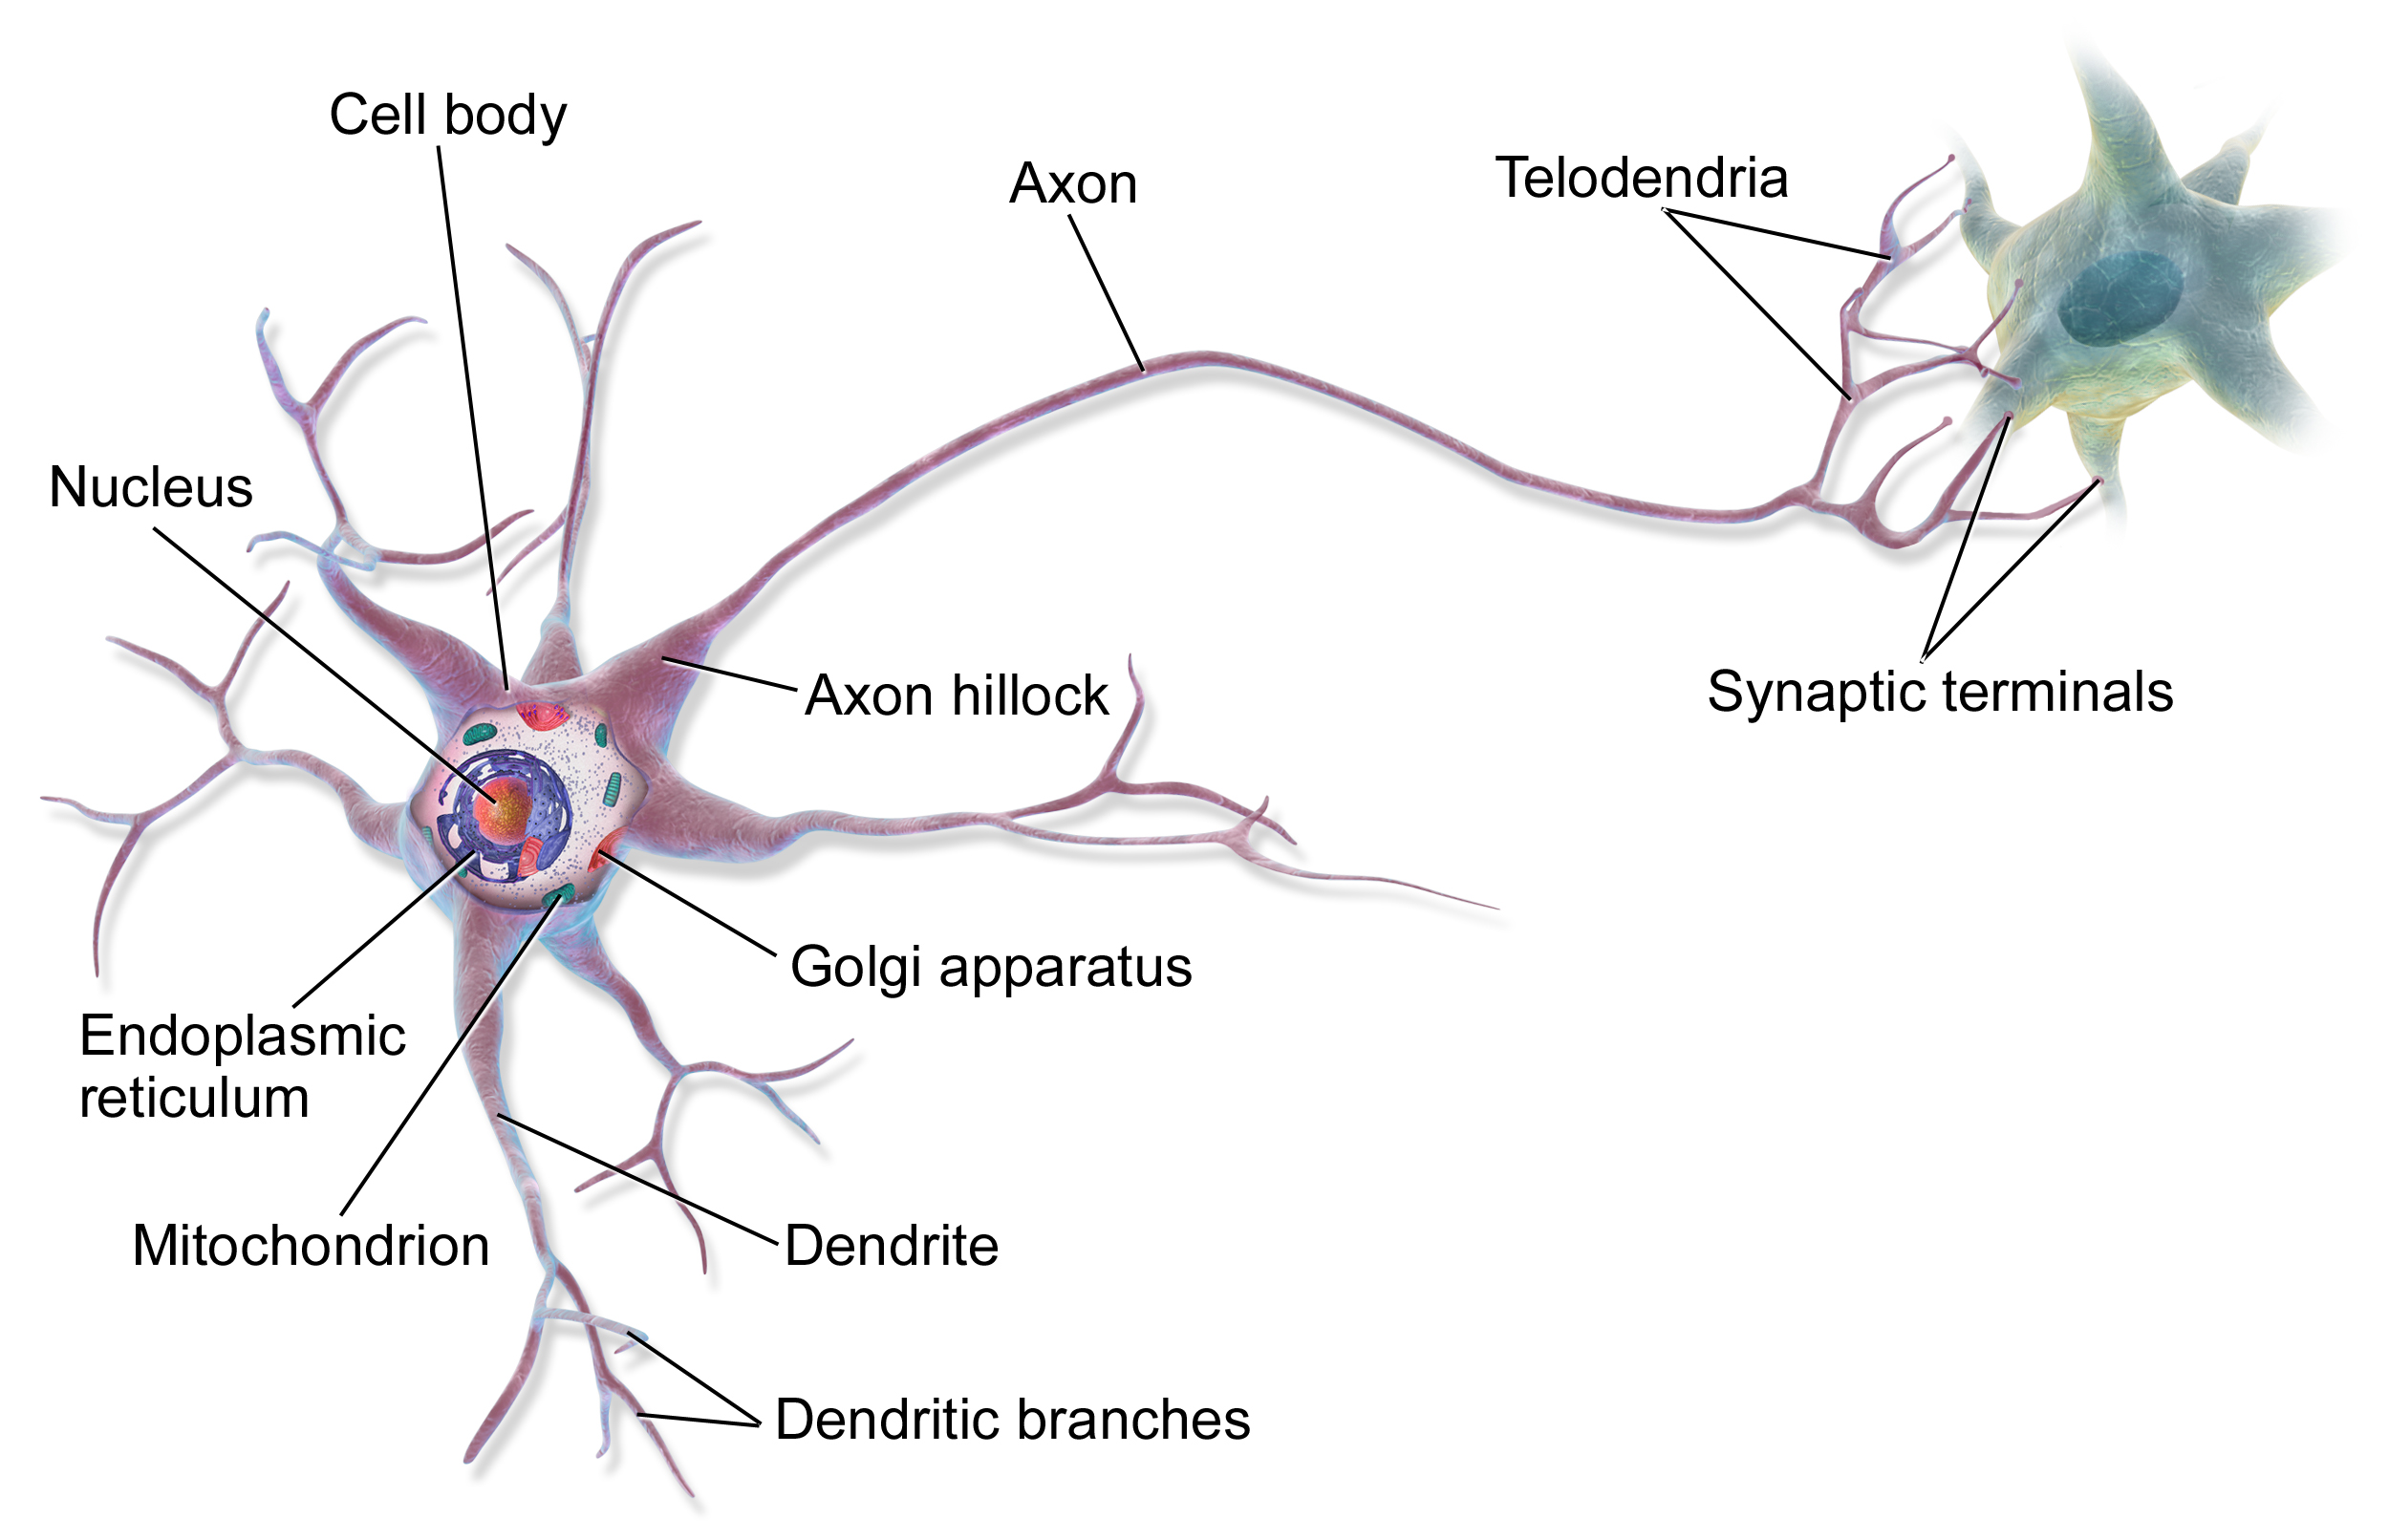
\includegraphics[width=0.3\textwidth]{neuron-detail}};
	\end{tikzpicture}
	
\end{frame}

\begin{frame}
	\frametitle{Computationalism}
	\framesubtitle{The Connectionist Computational Paradigm}
	\begin{figure}
		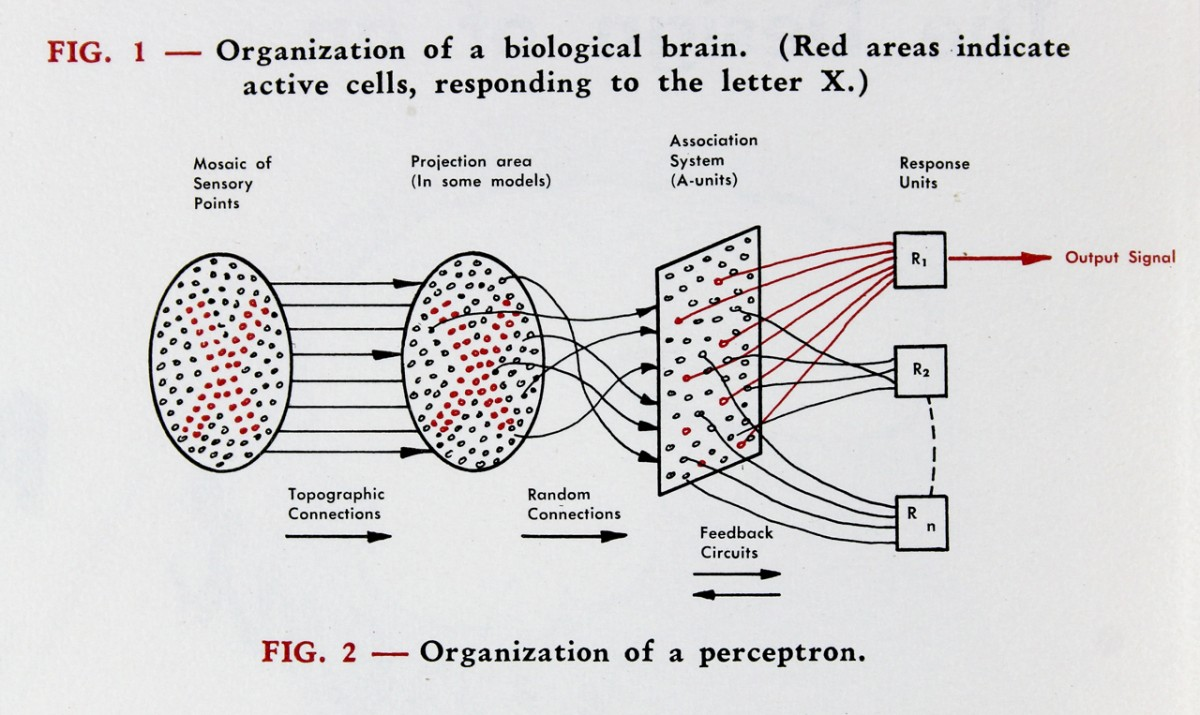
\includegraphics[width=0.75\textwidth]{perceptron_org}
		\caption{Von Frank Rosenblatt}
	\end{figure}
\end{frame}

\section{Feedward Neural Networks}
\begin{frame}
	\frametitle{Feedward Neural Networks}
	\begin{figure}
	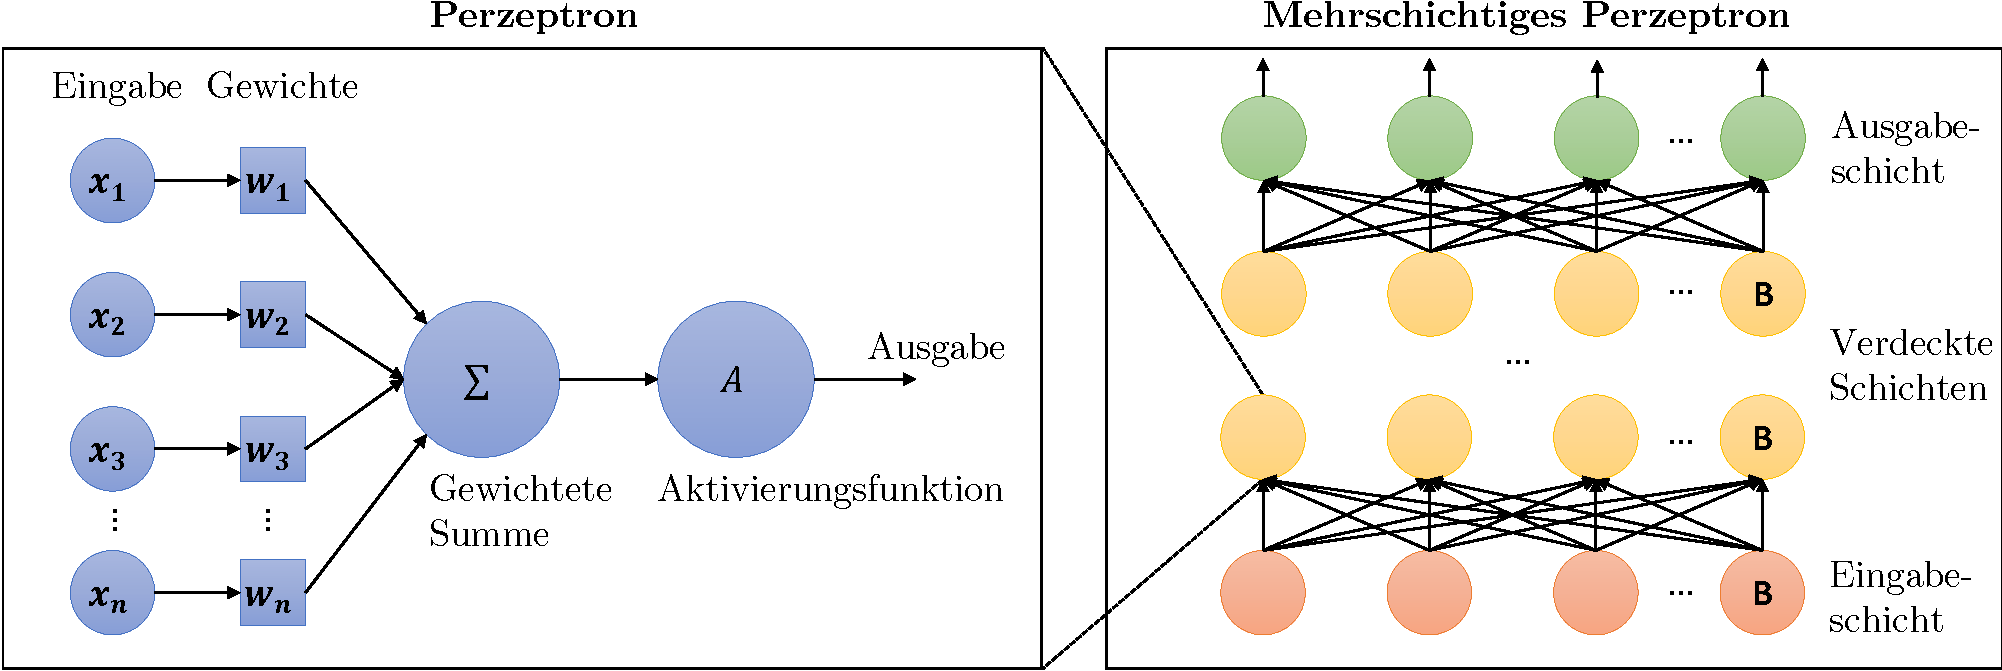
\includegraphics[width=1.0\textwidth]{perzeptron.pdf}
\end{figure}
\end{frame}

\begin{frame}
	\frametitle{Feedward Neural Networks}
	Ein paar Fakten:
	\begin{enumerate}[label=$\bullet$]
		\item Erste Einführung im Jahr 1943 und erste Erfolge bis in die 1990er
		\item Neuronale Netze sind abstrakte, vereinfachte Umsetzungen der Verknüpfung biologischer Neuronen.
		\item Sie können im Prinzip \hl{jede Funktion} ($\mathbb{R}^m \rightarrow \mathbb{R}^m$) annähern!
		\item Ausgabe ist \hl{probabilistisch}!
	\end{enumerate}
\end{frame}

%\begin{frame}
%	\frametitle{Feedward Neural Networks}
%	Ein paar Annahmen:
%	\begin{enumerate}[label=(\arabic*)]
%		\item Funktionale Einheiten (Neuronen) operieren alle ähnlich
%		\item Muster von Verbindungen im Netzwerk sind zentral für die Bestimmung wie Informationen verarbeitet werden
%	\end{enumerate}
%\end{frame}

\begin{frame}
	\frametitle{Feedward Neural Networks}
	\framesubtitle{Perzeptron}
	Basiselement eines neuronalen Netzes ist das \term{Perzeptron}, das zu mehrschichtigen Architekturen (daher das Deep in Deep Learning) kombiniert werden kann.
	\begin{figure}
		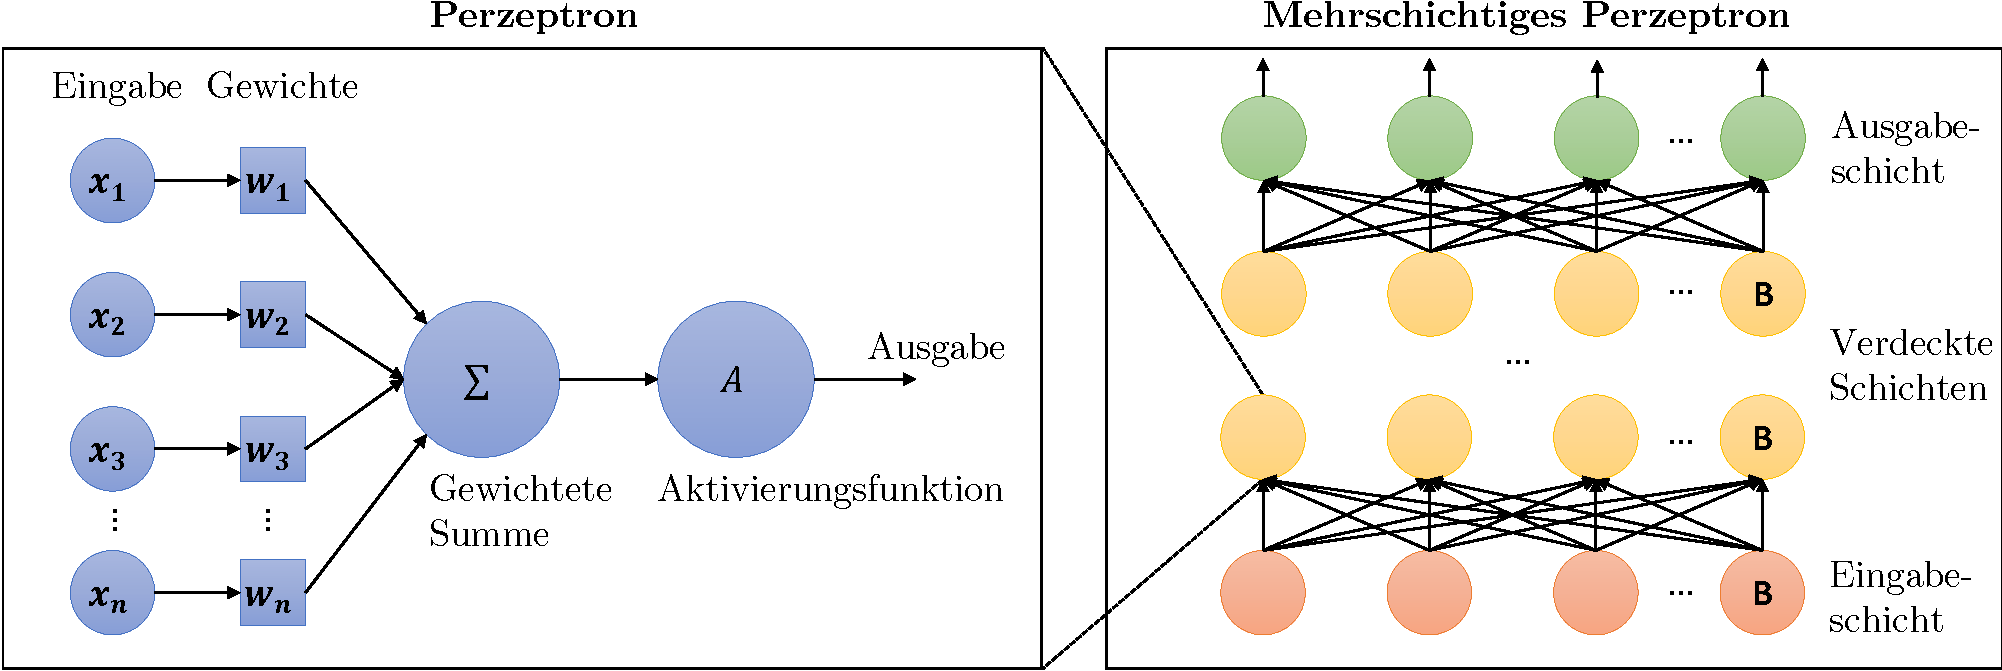
\includegraphics[width=1.0\textwidth]{perzeptron.pdf}
	\end{figure}
\end{frame}

\begin{frame}
	\frametitle{Feedward Neural Networks}
	\framesubtitle{Aktivierungsfunktion}
	Durch die \term{Aktivierungsfunktion} wird die Nicht-Linearität ermöglicht.
	\begin{figure}
		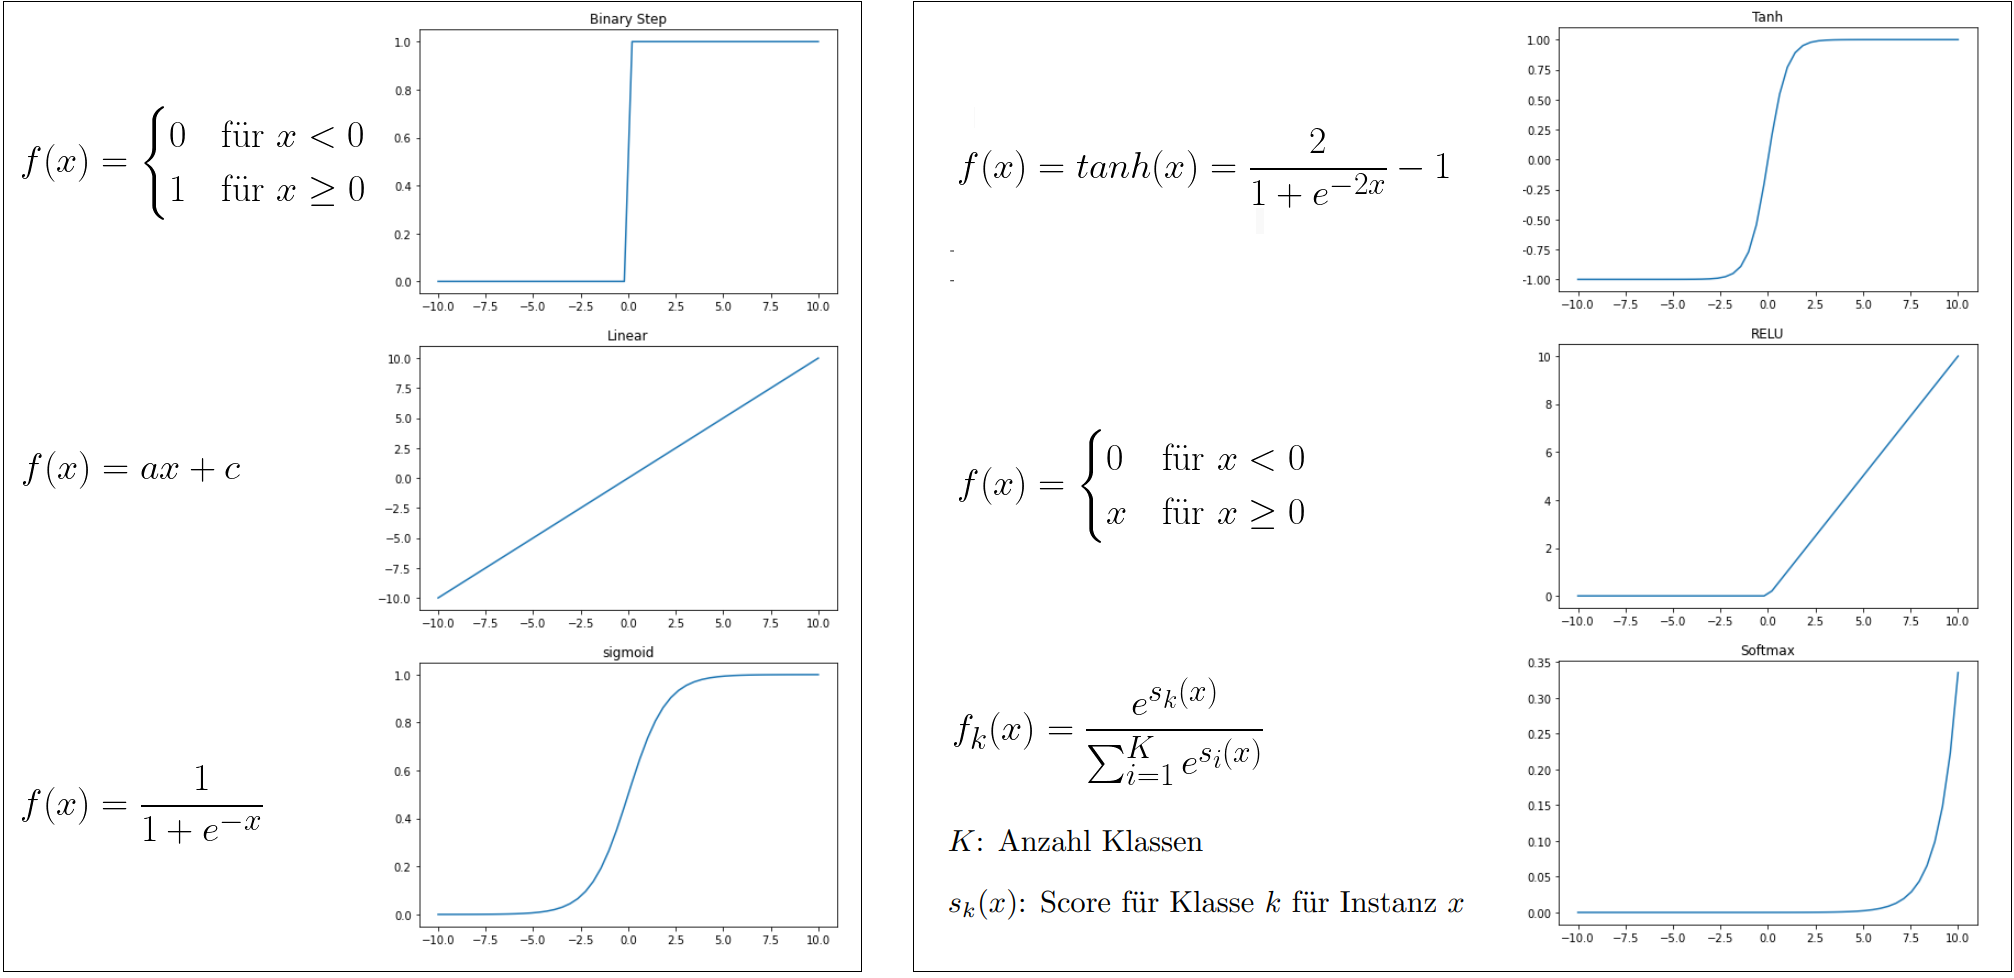
\includegraphics[width=0.9\textwidth]{activations.png}
	\end{figure}
\end{frame}

\begin{frame}
	\frametitle{Feedward Neural Networks}
	\framesubtitle{Einfachstes Neuronales Netz}
	Eine (\term{parametrisierbare}) Geradengleichung 
	
	$$h_\theta(x) = w_0 \cdot x + w_1$$
	
	mit den Gewichten $w_0, w_1 \in \theta$ ist im Prinzip ein \term{neuronales Netz}:
	
	\begin{figure}[b]
		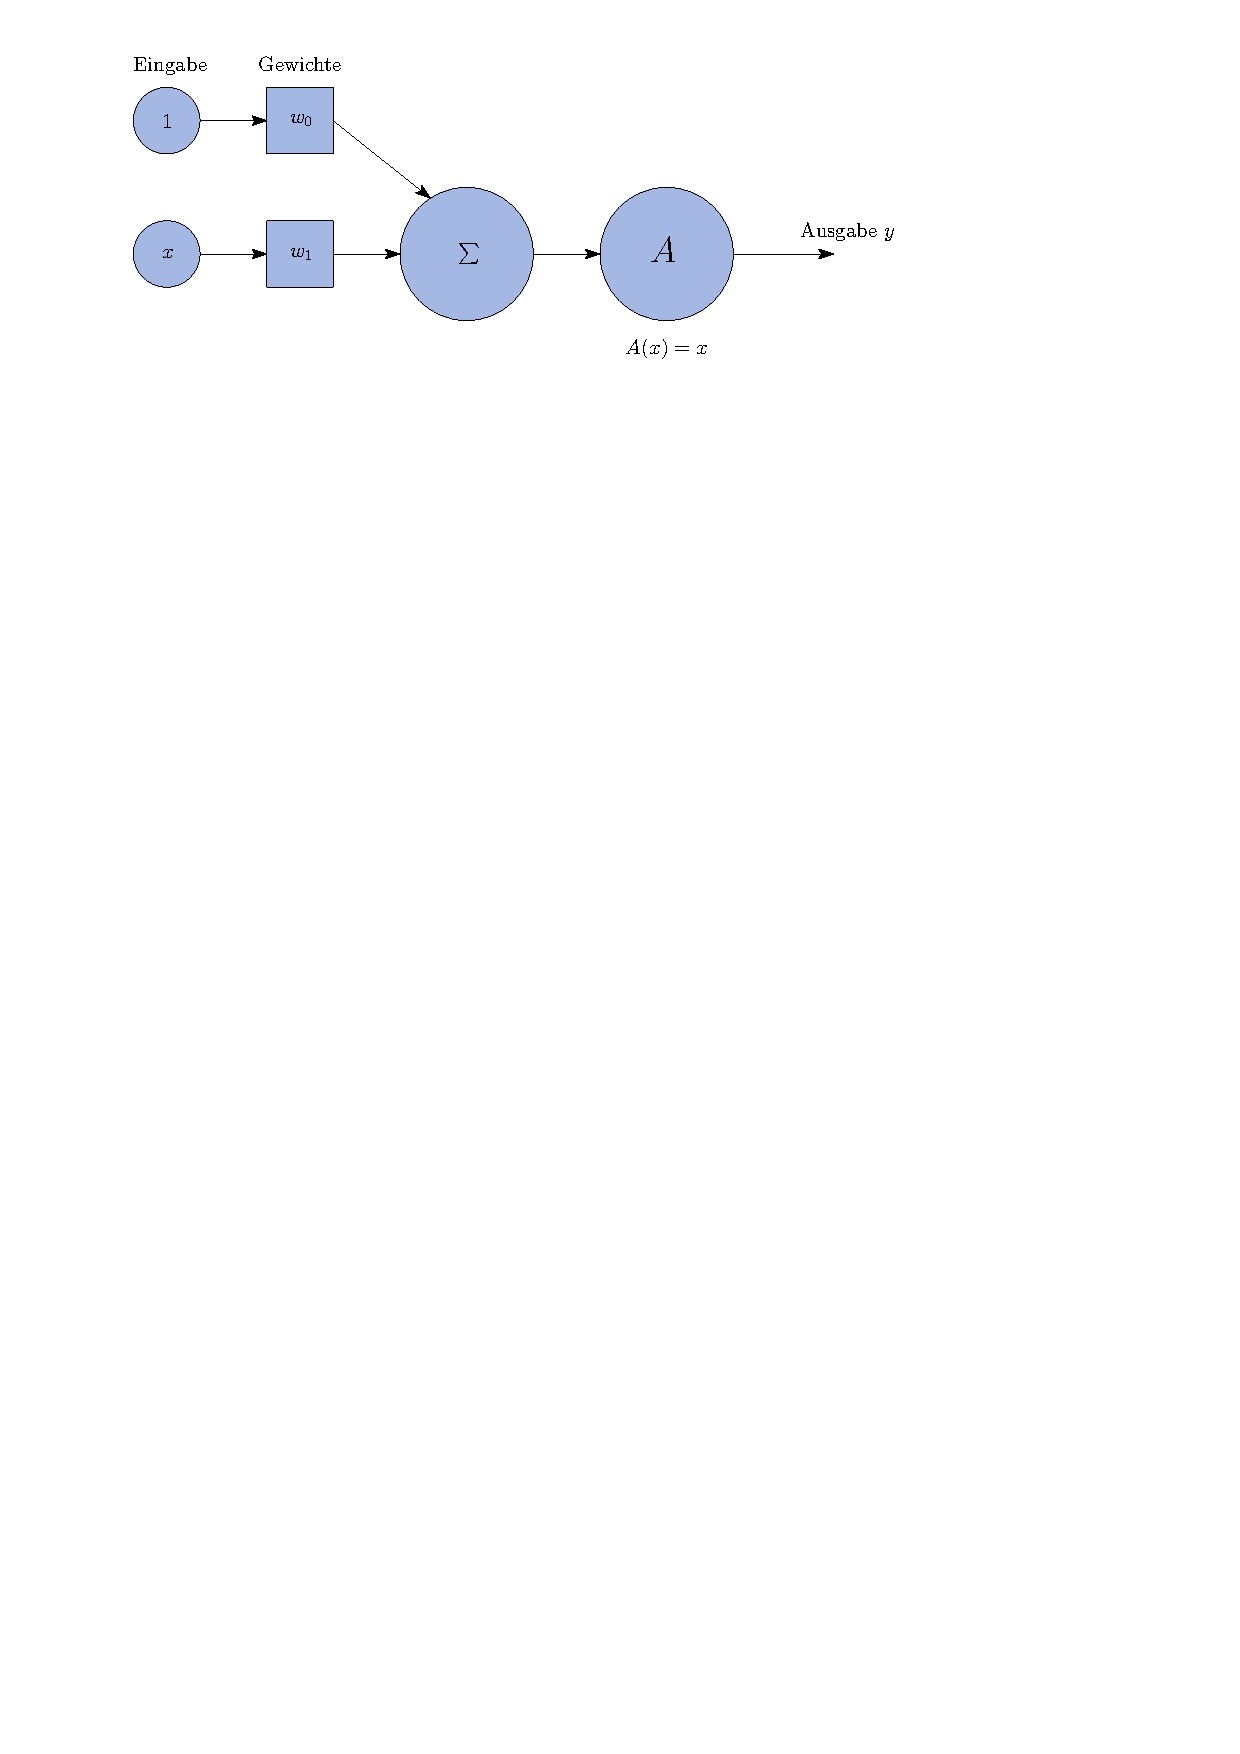
\includegraphics[width=0.55\textwidth]{simple-ann.pdf}
	\end{figure}
	
	Nehmen wir nun an wir hätten Datenpunkte (Antworten) $(x_1, y_1) = (0,0)$ und $(x_2, y_2) = (1,1)$ gegeben.
\end{frame}

\begin{frame}
	\frametitle{Feedward Neural Networks}
	\framesubtitle{Training}
	
	\begin{definition}[(informell) Training]
		Beim Training eines neuronalen Netzes suchen wir Parameter $\theta$ (hier $w_0, w_1$), sodass der Fehler zwischen unserem Netz hier
		(hier $h_\theta(x_1)$, $h(x_2)$) und den Trainingsdatenpunkten (hier $y_1, y_2$) möglichst klein wird.
	\end{definition}
	
	\vspace{1cm}
	Wir kalibrieren unsere Neuronen sodass diese bei bestimmten Eingaben 'richtig' feuern.
	
\end{frame}

\begin{frame}
		\frametitle{Feedward Neural Networks}
		\framesubtitle{Training (Gradient Descent)}
		Wir haben Antworten: $(x_1, y_1) = (0,0)$ und $(x_2, y_2) = (1,1)$. Initialisiere Parameter zufällig, z.B.: $w_0 = 3, w_1 = 6$
		\begin{equation*}
			h_\theta(x) = \underbrace{3}_{w_0} x + \underbrace{6}_{w_1}
 		\end{equation*}
 		Daraus ergeben sich Fehler:
 		\begin{equation*}
 			\begin{split}
 				 y_1 - h_\theta(x_1) = y_1 - h_\theta(0) = 0 - 6 = -6\\
 				 y_2 - h_\theta(x_2) = y_2 - h_\theta(1) = 1 - 9 = -8
 			\end{split}
 		\end{equation*}
 		
		Wir suchen die \term{Parameter} $\theta$, sodass der Fehler (oder auch die \term{Kostenfunktion})
		\begin{equation*}
			J(\theta) = (y_1 - h_\theta(x_1))^2 + (y_1 - h_\theta(x_2))^2
		\end{equation*}
		minimal wird!
\end{frame}


\begin{frame}
	\frametitle{Feedward Neural Networks}
	\framesubtitle{Training (Gradient Descent)}
	Berechne Gradient des Fehlers
	\begin{equation*}
		\begin{split}
			J(\theta) &= (y_1 - h_\theta(x_1))^2 + (y_1 - h_\theta(x_2))^2\\
			%&= \frac{1}{2} (0 - \theta_1 \cdot x_1 - \theta_2)^2 + (1 - \theta_1 \cdot x_2 - \theta_2)^2\\
			%&= \frac{1}{2} (0 - \theta_1 \cdot 0 - \theta_2)^2 + (1 - \theta_1 \cdot 1 - \theta_2)^2\\
			&= -\frac{1}{2} w_1^2 + \frac{1}{2}(1 - w_1 - w_0)^2
		\end{split}
	\end{equation*}
	wobei wir nach den \term{Parametern} ableiten:
	\begin{equation*}
		\nabla J(\theta) = \begin{pmatrix}
			\frac{\partial J}{\partial w_0} \\
			\frac{\partial J}{\partial w_1} \\
		\end{pmatrix} = \begin{pmatrix}
			w_0 + w_1 - 1  \\
			w_0 - 1  \\
		\end{pmatrix} = \begin{pmatrix}
			8  \\
			2\\
		\end{pmatrix}
	\end{equation*}
	Wir können nun iterativ neue \term{Parameter} berechnen:
	\begin{equation*}
		\theta^{i+1} = \theta^{i} - \mu \cdot \nabla J(\theta^i)
	\end{equation*}
	bis $ \nabla J(\theta^i) \approx 0$ wird.
\end{frame}

\begin{frame}
	\frametitle{Feedward Neural Networks}
	\framesubtitle{Kettenregel}
	Wir haben die Kostenfunktion
	\begin{equation*}
		\begin{split}
		J(\theta) &= (\yy_1 - h_\theta(\xx_1))^2 + (\yy_1 - h_\theta(\xx_2))^2 + \ldots + (\yy_n - h_\theta(\xx_m))^2\\
		&= \sum\limits_{i = 1}^m (\yy_i - h_\theta(\xx_i))^2
		\end{split}
	\end{equation*}
	und wollen iterativ unsere \term{Parameter} $\theta$ anpassen:
	\begin{equation*}
		\theta^{i+1} = \theta^{i} - \mu \cdot \nabla J(\theta^i)
	\end{equation*}
	bis $ \nabla J(\theta^i) \approx 0$ wird. Wir brauchen demnach die Gradienten
	\begin{equation*}
		\nabla J(\theta^i)
	\end{equation*}
\end{frame}

%\begin{frame}
%	\frametitle{Feedward Neural Networks}
%	\framesubtitle{Kettenregel}
%	\begin{equation*}
%		\nabla J(\theta^i) = \nabla \left( \sum\limits_{i = 1}^m (\yy_i - h_\theta(\xx_i))^2 \right)
%	\end{equation*}
%\end{frame}

\begin{frame}
	\frametitle{Feedward Neural Networks}
	\framesubtitle{Training (Gradient Descent)}
	\begin{figure}
	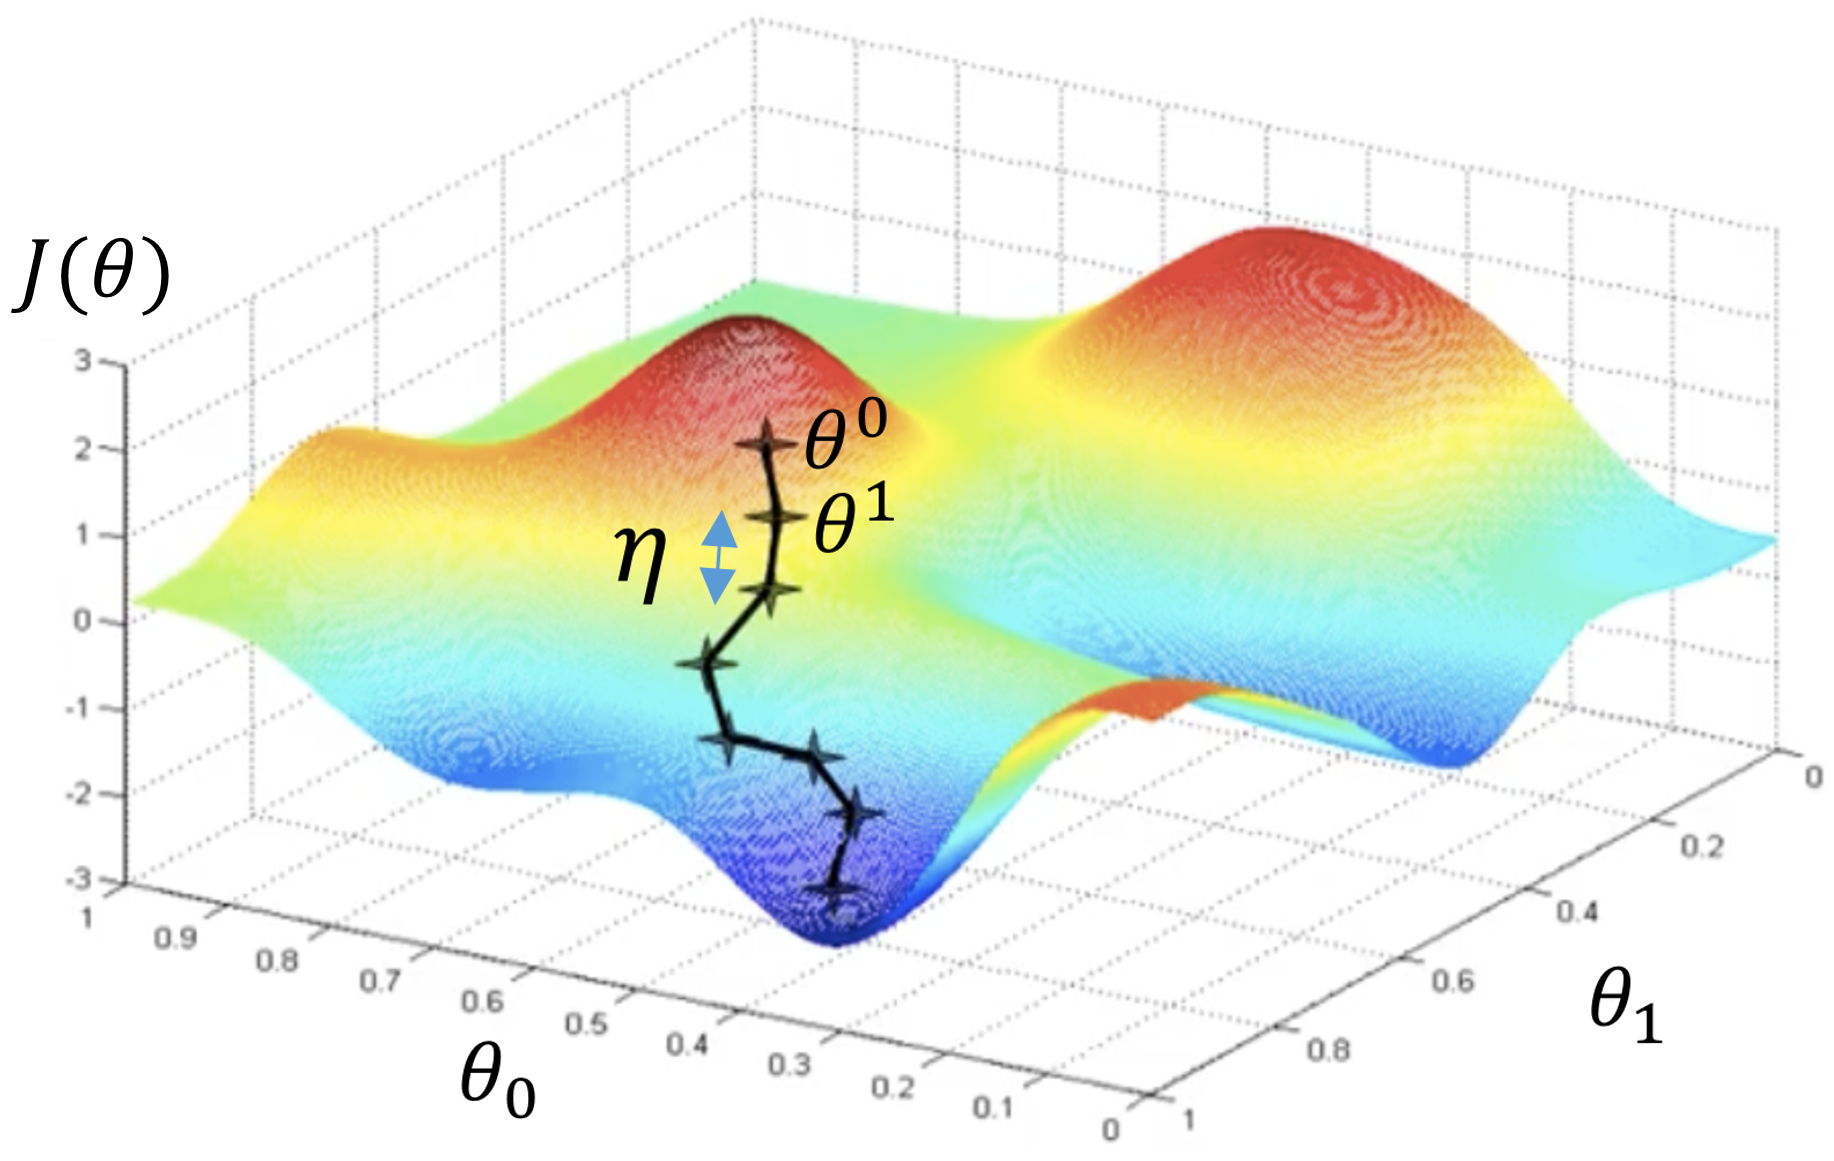
\includegraphics[width=0.7\textwidth]{gd_example.png}
\end{figure}
\end{frame}

\section{Training im Detail}
\begin{frame}
	\frametitle{Training im Detail}
	\framesubtitle{Ablauf}
	\begin{columns}
		\begin{column}{0.5\textwidth}
			\hl{Trainingsablauf}:
			\begin{enumerate}[label=(\arabic*)]
				\uncover<2->{\item Vorhersage $\mathbf{\hat{y}} = h_{\theta^i}(\xx)$ berechnen}
				\uncover<3->{\item Fehler $J(\theta^i)$ berechnen $\nabla J(\theta^i)$ berechnen}
				\uncover<4->{\item Gradient(en) des Fehlers bestimmen}
				\uncover<5->{\item Parameter anpassen $\theta^{i+1} = \theta^{i} - \mu \cdot \nabla J(\theta^i)$}
			\end{enumerate}
		\end{column}
		\begin{column}{0.5\textwidth}
			\only<2-3>{\begin{figure}
				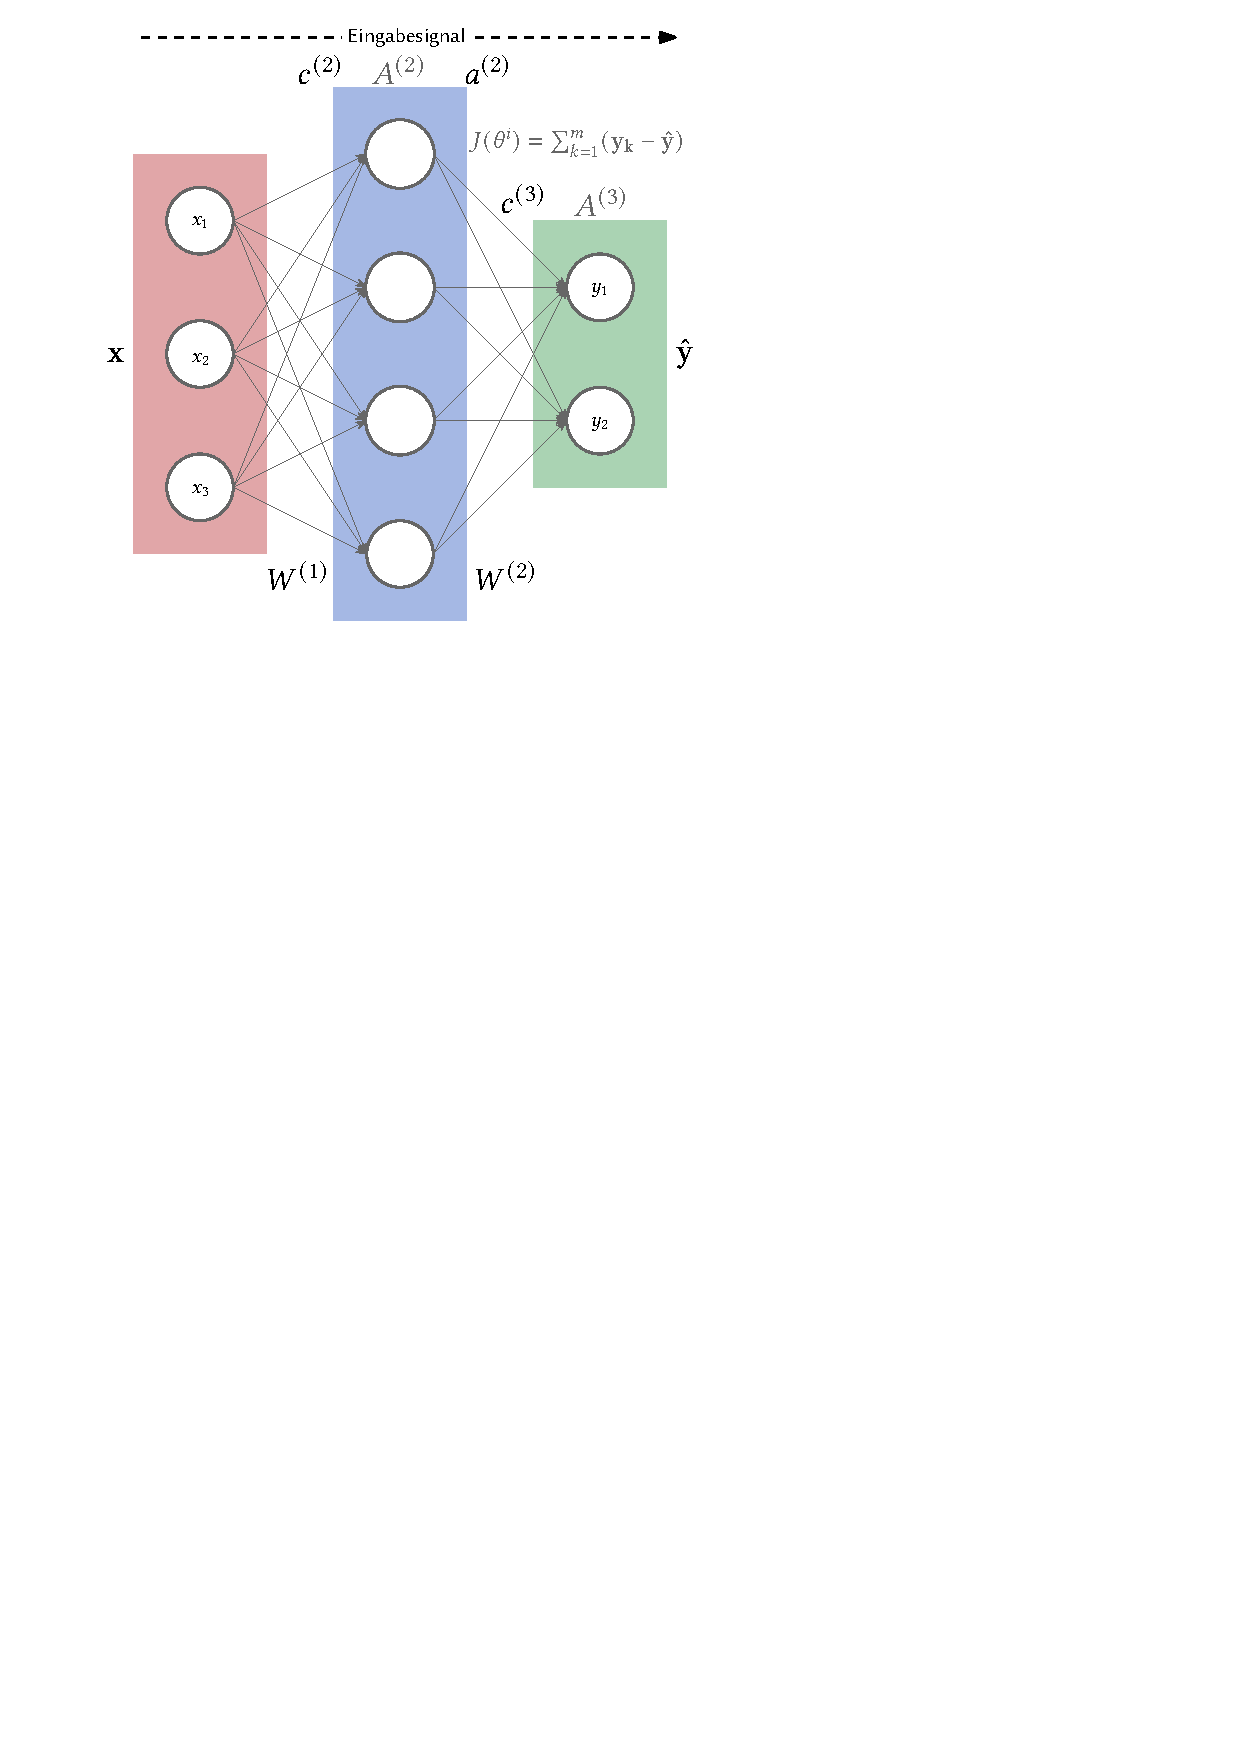
\includegraphics[scale=0.6]{forward}
			\end{figure}}
				\only<4-5>{\begin{figure}
					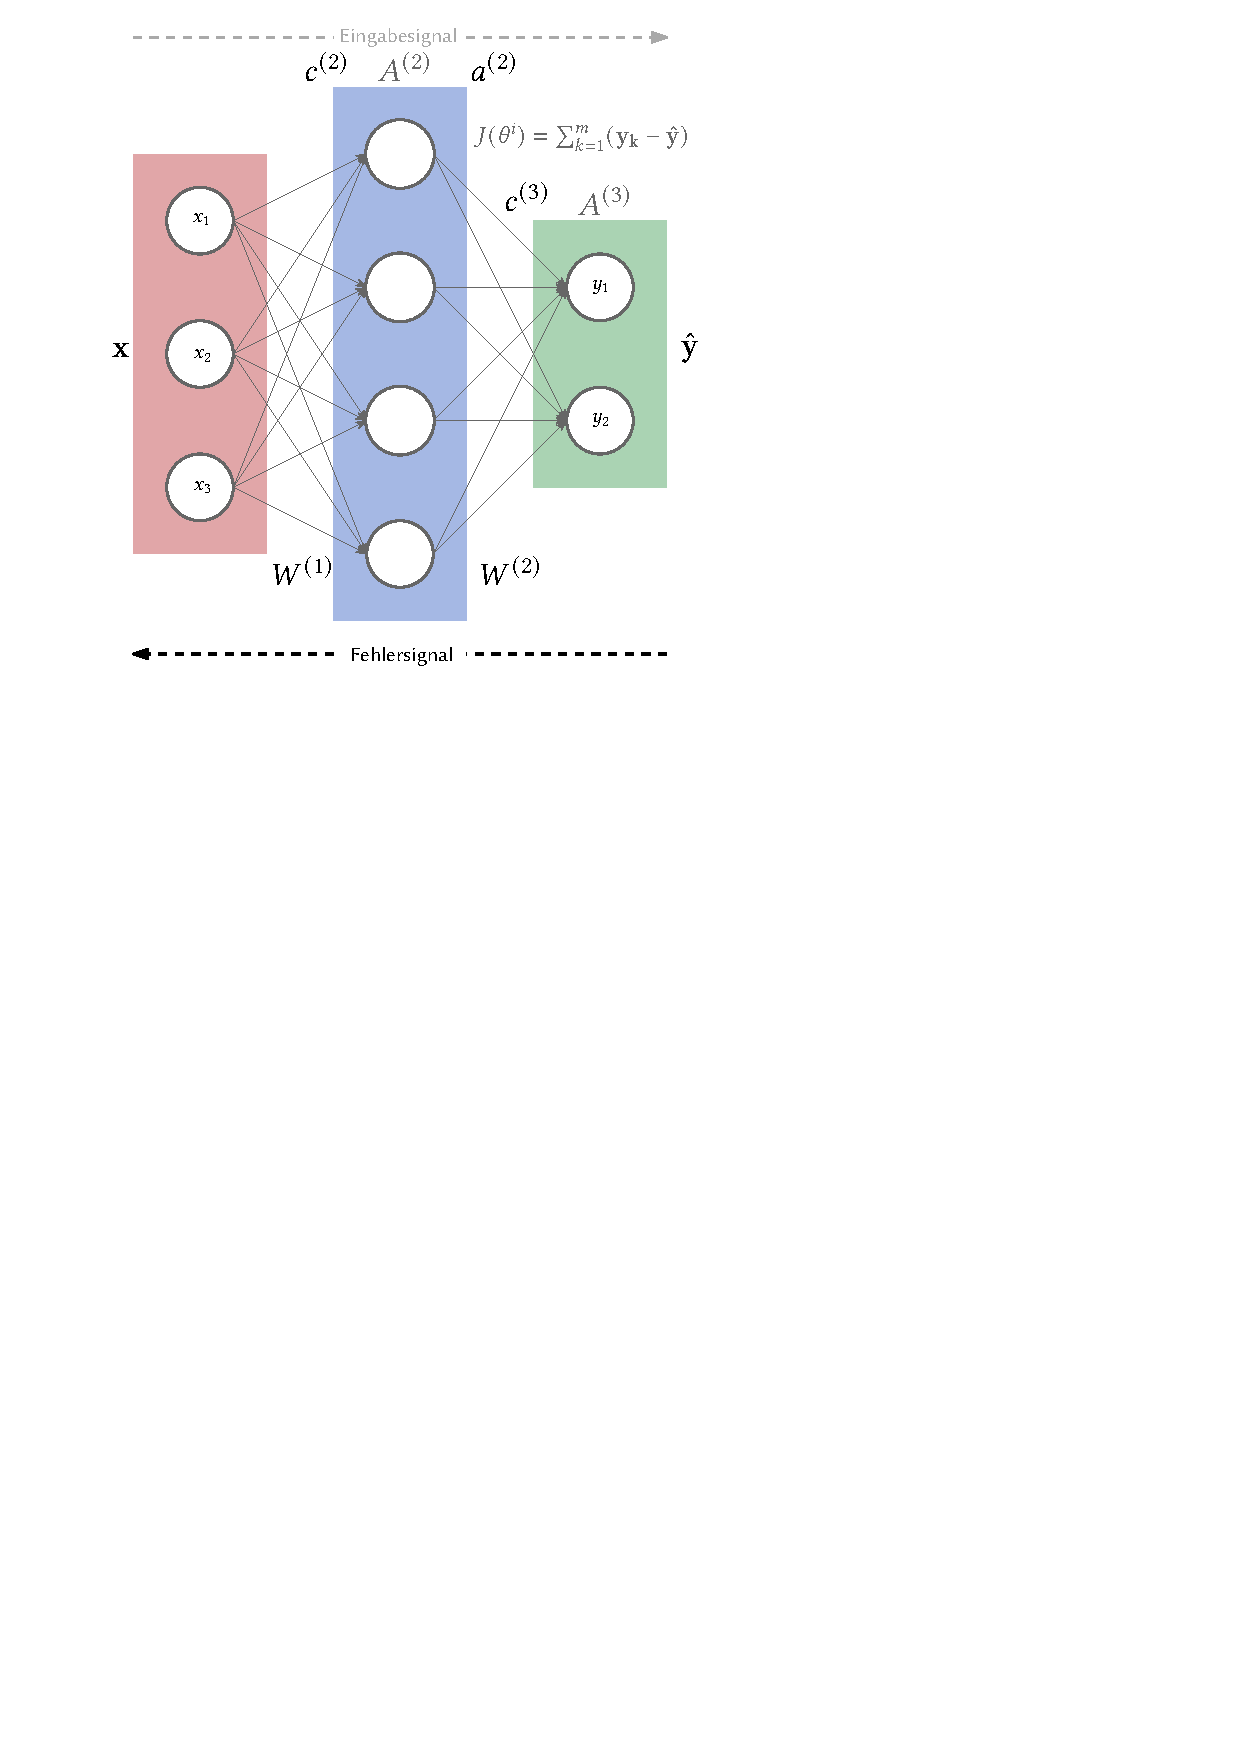
\includegraphics[scale=0.6]{backward}
			\end{figure}}
		\end{column}
	\end{columns}
\end{frame}

\begin{frame}
	\frametitle{Training im Detail}
	\framesubtitle{Vorhersage berechnen}
	\begin{columns}
		\begin{column}{0.5\textwidth}
			\hl{Vorhersage berechnen}:
			\begin{enumerate}[label=(\arabic*)]
				\uncover<2->{\item $c^{(2)} = \xx W^{(1)}, \text{ mit } W^{(1)} \in \mathbb{R}^{3 \times 4}$}
				\uncover<3->{\item $a^{(2)} = A^{(2)}(c^{(2)})$}
				\uncover<4->{\item $c^{(3)} = a^{(2)} W^{(2)}, \text{ mit } W^{(2)} \in \mathbb{R}^{4 \times 2}$}
				\uncover<5->{\item $\yy = A^{(3)}(c^{(3)})$}
			\end{enumerate}
		\end{column}
		\begin{column}{0.5\textwidth}
			\begin{figure}
					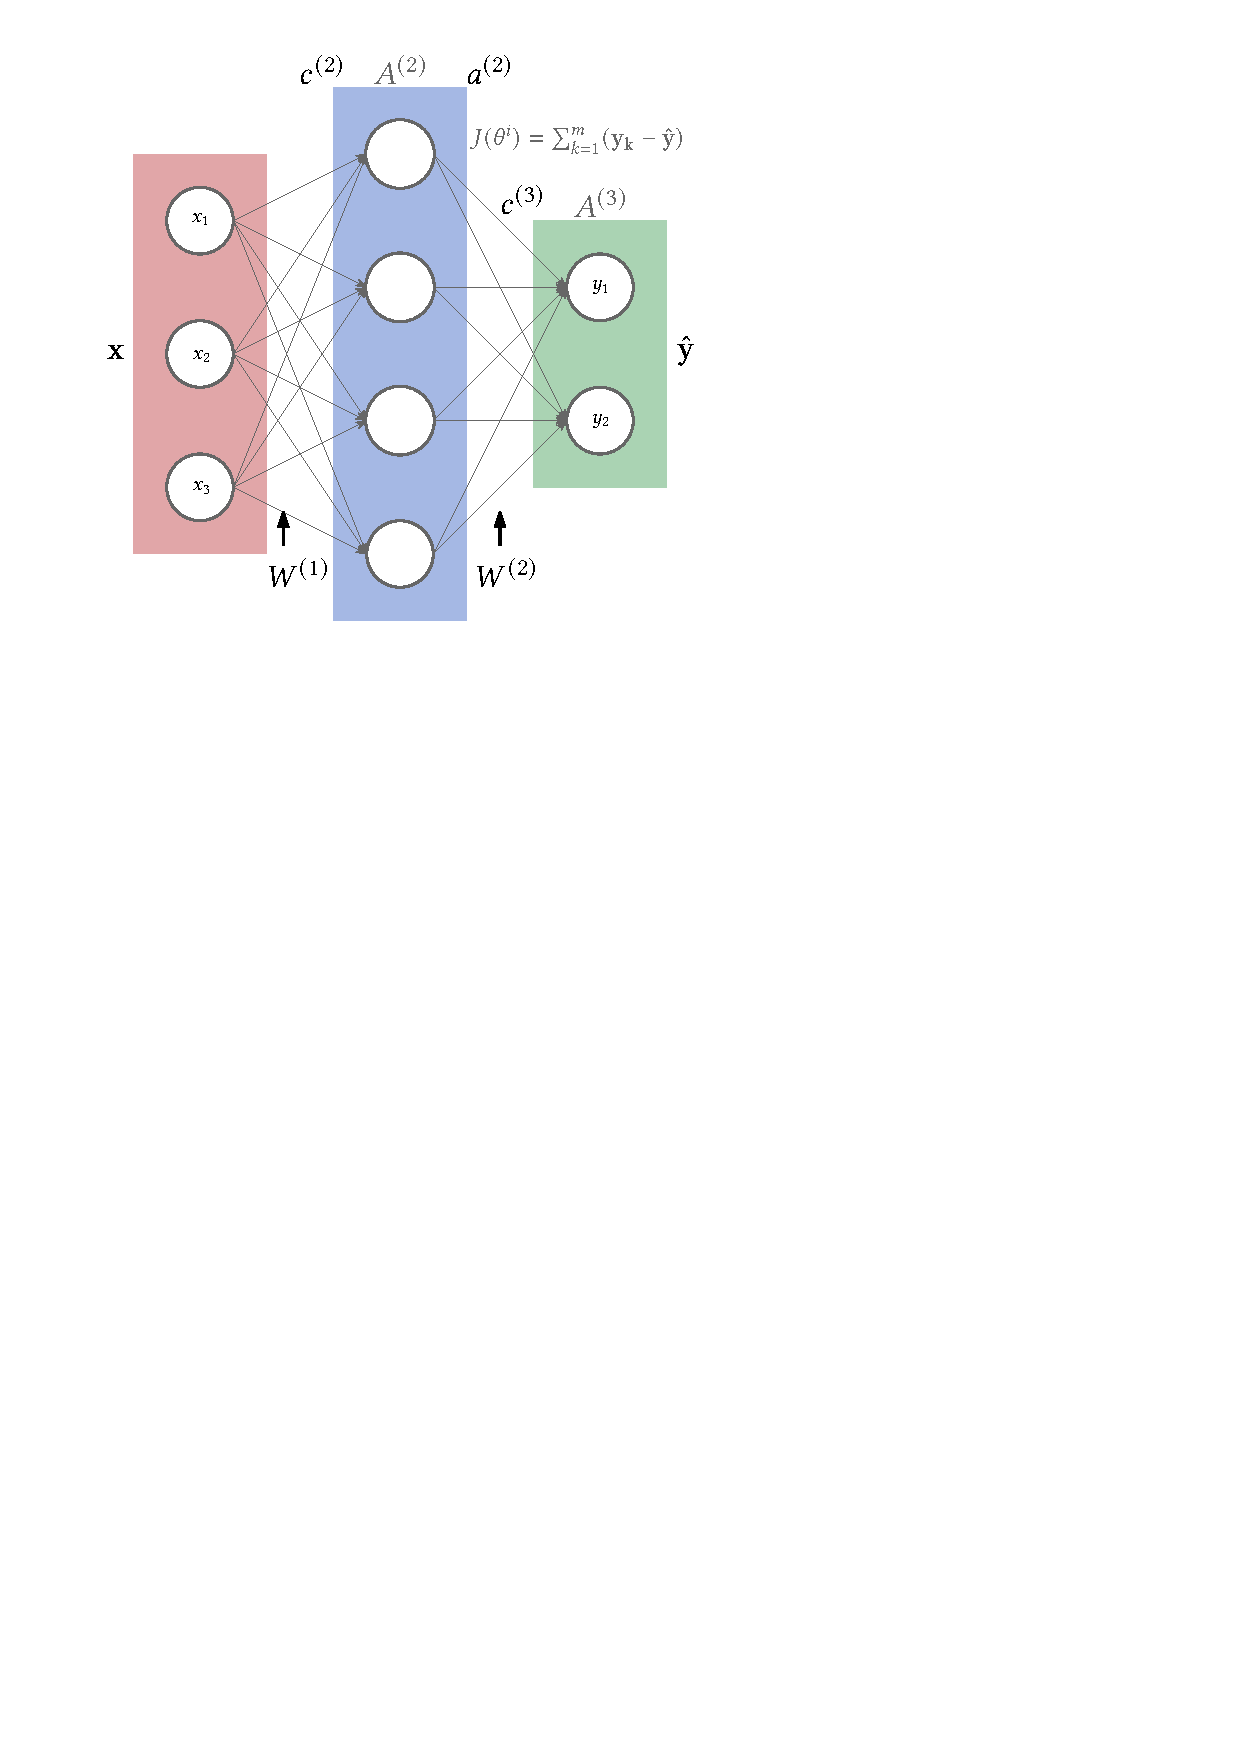
\includegraphics[scale=0.68]{fnn}
			\end{figure}
		\end{column}
	\end{columns}
\end{frame}


\begin{frame}[t]
	\frametitle{Training im Detail}
	\framesubtitle{Berechnung der Gradienten}
	\begin{columns}
		\begin{column}{0.5\textwidth}
			\hl{Gradient(en) des Fehlers bestimmen}:
			\only<2>{
				\begin{equation*}
				\frac{\partial f}{ \partial x} = \frac{\partial f}{ \partial q} \frac{\partial q}{\partial x}
			\end{equation*}
		Ist die Magie der Kettenregel. Beispiel:
		$f(x,y) = (x+y)^2$ wir setzen $q = (x+y)$.\\
		Dann können wir rechnen:
		$$ \frac{\partial f}{\partial x} = \frac{\partial q^2}{\partial q} \frac{\partial q}{\partial x} = 2q \cdot \frac{\partial (x+y)}{\partial x} = 2(x+y)$$
}%
			\only<3>{\begin{equation*}
				\nabla J(\theta) \text{ d.h. } \frac{\partial J}{\partial W^{(k)}}
			\end{equation*}}
			\only<4>{\begin{equation*}
						\begin{split}
							 \frac{\partial J}{\partial W^{(2)}} &= \frac{\partial J}{\partial \mathbf{\hat{y}}} \frac{\partial \mathbf{\hat{y}}}{\partial W^{(2)}}\\
							  &= \frac{\partial J}{\partial \mathbf{\hat{y}}} \frac{\partial \mathbf{y}^{(3)}}{\partial c^{(3)}}  \frac{\partial c^{(3)}}{\partial W^{(2)}}
						\end{split}
			\end{equation*}}
			\only<5>{\begin{equation*} 
				\begin{split}
					\frac{\partial J}{\partial W^{(1)}} &= \frac{\partial J}{\partial a^{(2)}} \cdot \frac{\partial a^{(2)}}{\partial c^{(2)}} \frac{\partial c^{(2)}}{\partial W^{(1)}}\\
					&= \frac{\partial J}{\partial \mathbf{\hat{y}}} \frac{\partial \mathbf{\hat{y}}}{\partial c^{(3)}} \frac{\partial c^{(3)}}{\partial a^{(2)}} \cdot \frac{\partial a^{(2)}}{\partial c^{(2)}} \frac{\partial c^{(2)}}{\partial W^{(1)}}
				\end{split}
		\end{equation*}}
		\end{column}
		\begin{column}{0.5\textwidth}
			\begin{figure}
				\includegraphics[scale=0.65]{normal}
			\end{figure}
		\end{column}
	\end{columns}
\end{frame}

%\begin{frame}
%	\frametitle{Transfer Learning}
%	\framesubtitle{Parametertransfer}	
%	\begin{figure}
%		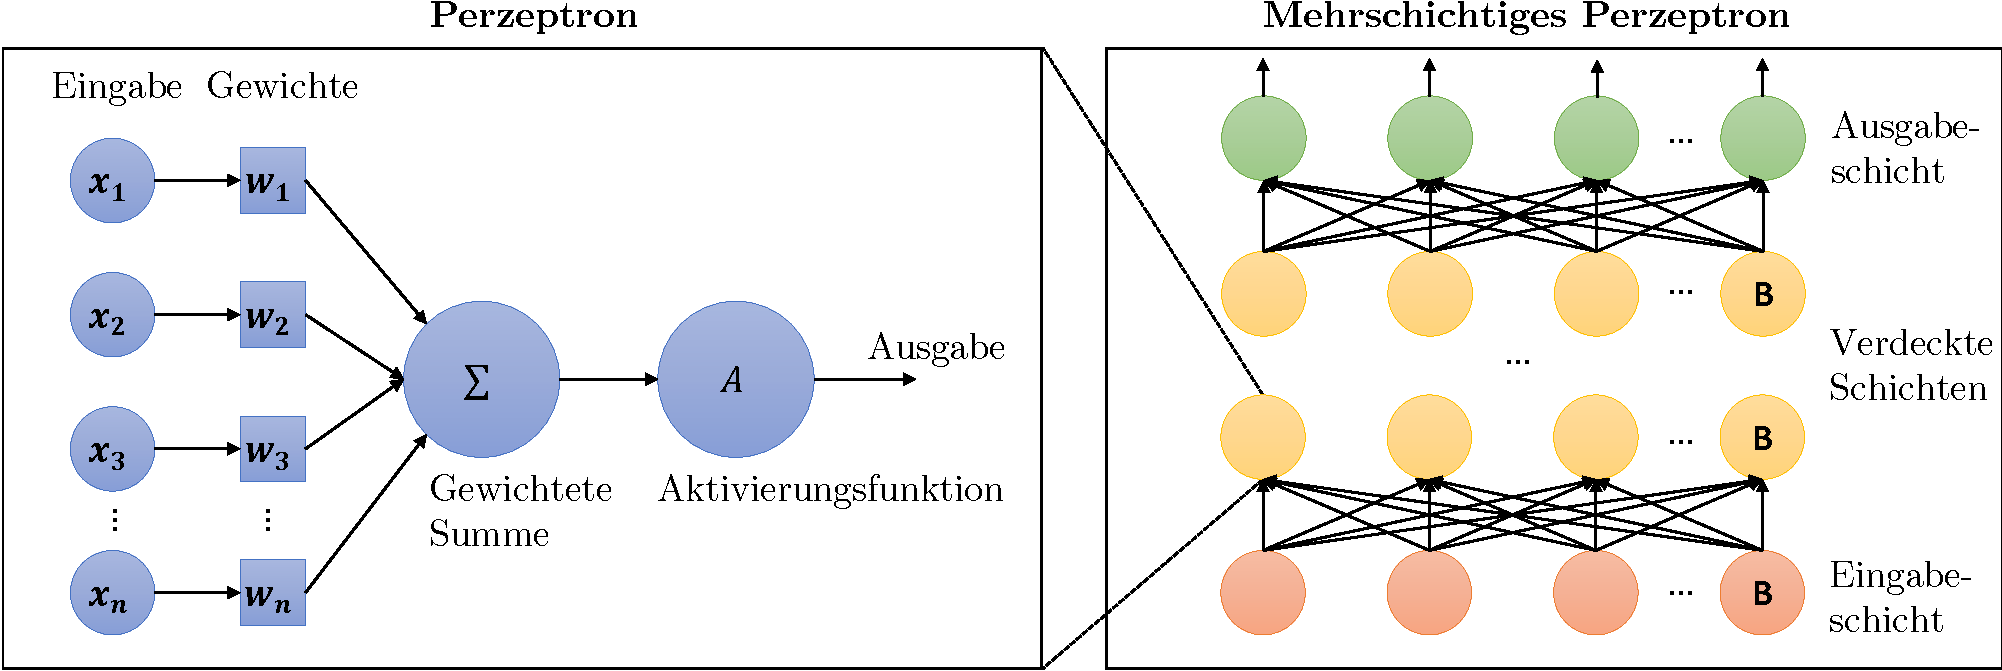
\includegraphics[width=1.0\textwidth]{perzeptron.pdf}
%	\end{figure}
%\end{frame}


\begin{frame}
	\frametitle{Feedward Neural Networks}
	\framesubtitle{Training (Gradient Descent)}
	\hl{Probleme}:
	\begin{enumerate}[label=$\bullet$]
		\item Black Box Problem
		\item Berechnungsaufwand (besonders beim Training) $\Rightarrow$ hoher Ressourcenverbrauch
		\item Je komplexer das Netz desto mehr Daten werden fürs Training gebraucht
		\item Keine Garantie für Korrektheit
		\item Können kaum mit zeitlichen Abhängigkeiten umgehen (Sprache, Melodien, usw.)
		\item Qualität hängt von den Trainingsdaten und der ausgewählten Architektur zusammen (induzierte Verzerrung)
	\end{enumerate}
\end{frame}

\begin{frame}
	\frametitle{Feedward Neural Networks}
	\framesubtitle{Networks and Brains}
	\begin{quoting}
		``Although neural networks may initially seem biologically plausible as they 'take inspiration from the brain' many of the established technniques used by neural networks modellers (especially the backpropagation of errors) are not biologically realistic.'' -- A. Browne 
	\end{quoting}
\end{frame}


%\begin{frame}
%	Wir möchten einen Algorithmus $h$ mit einem \term{Trainingsdatensatz} $\dataset$ (Erfahrung) ``trainieren'', 
%	ein \term{Zuordnungsproblem} zwischen Ein- und Ausgabe (Aufgabe) möglichst gut (Leistungskriterium) lösen:
%	\begin{figure}
%		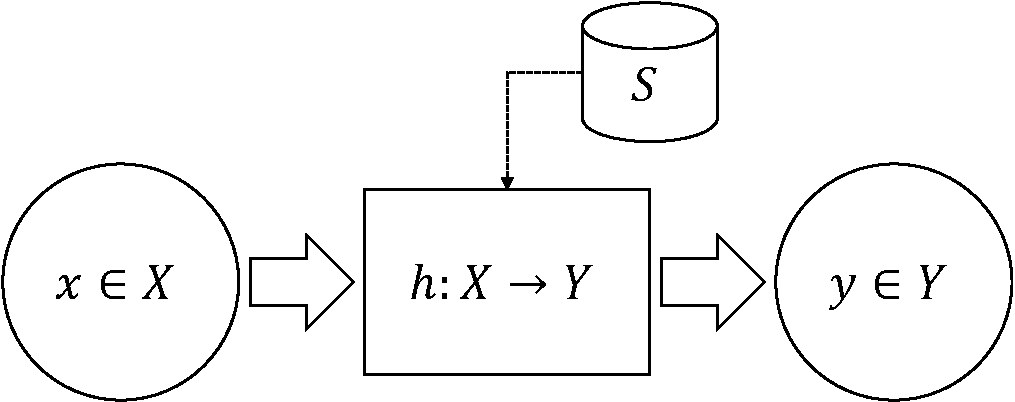
\includegraphics[width=0.4\textwidth]{supervised}
%	\end{figure}
%	\vspace{0.5cm}
%	\begin{enumerate}[label=$\bullet$]
%		\item Eingabe: $\xx \in \features$, Ausgabe: $y \in \labels$.
%		\item $\features$ wird auch \term{Merkmalsraum} genannt, $\labels$ ist der sog. \term{Labelraum}.
%		\item Trainingsdatensatz $\dataset = \{(\xx_{1},y_{1}),...,(\xx_{m},y_{m})\}$ mit $m$ Elementen.
%	\end{enumerate}
%\end{frame}
%
%\begin{frame}
%	\begin{Beispiel}[Problem]
%		Erkennung von unterschiedlichen Kleidungstypen auf Farbbildern.
%		\begin{enumerate}[label=$\bullet$]
%			\item Eingabe: $\xx \in \features$ Farbbild im Raum der möglichen Farbbilder
%			\item Ausgabe: $y \in \labels$ Kleidungstyp (T-Shirt, Pullover, usw.)
%			\item Trainingsdatensatz $\dataset = \{(\xx_{1},0),...,(\xx_{m},1)\}$ Bilder mit der Information des Kleidungstyps, z.B. $0$ entspricht 'Pullover'.
%		\end{enumerate}
%	\end{Beispiel}
%\end{frame}
%
%\begin{frame}
%		Wir unterscheiden zwei Zuordnungsproblemtypen:
%	\begin{enumerate}[label=$\bullet$]
%		\item \term{Klassifikation:} $\labels$ ist endlich und diskret: Ausgabe ist eine Klasse $y$ aus einer Menge vorher definierter Klassen $\labels$.
%		\item \term{Regression:} $\labels$ ist kontinuerlich: Ausgabe ist ein kontinuerlicher Wert.
%	\end{enumerate}
%	\vspace{0.5cm}
%	\begin{Beispiel}[Klassifikation]
%		Speisepilzklassifikation auf Basis von Fotos.
%	\end{Beispiel}
%	
%	\begin{Beispiel}[Regression]
%		Temperaturvorhersage auf Basis der Temperatur der letzten Tage.
%	\end{Beispiel}
%\end{frame}
%
%\begin{frame}
%	\begin{enumerate}[label=$\bullet$]
%	\item Unser Algorithmus $h$ nutzt eine Reihe von Parametern $\theta \in \Theta$ innerhalb seiner Berechnungsschritte (ab jetzt also $h_{\theta}$).
%	\item Wir nennen $h_{\theta}$ ab jetzt ein \term{Modell} und $\theta$ \term{Modellparameter} (auch: \term{Hypothese}). 
%	\item Die durch ein Modell gefundene Lösung $\hat{y} = h_{\theta}(x)$ des Zuordnungsproblems ist eine \term{Prädiktion}.
%\end{enumerate}
%
%\begin{definition}[Lernen / Training]
%	Training bedeutet, diejenigen Modellparameter $\theta \in \Theta$ zu finden, 
%	sodass das Modell $h_{\theta}$ die im Trainingsdatensatz gegebenen Zuordnungen möglichst gut prädizieren kann.  
%\end{definition}
%\end{frame}

\begin{frame}[allowframebreaks]
	\frametitle{Referenzen}
	{\scriptsize% dirty fix for the non-chapter bib
		\bibliographystyle{apalike}
		\bibliography{./../../literature/references.bib}}
\end{frame}

\end{document}